\documentclass[a4paper]{article}
\PassOptionsToPackage{table}{xcolor}
\usepackage[T1]{fontenc}   % lets XeLaTeX use the template's Type-1 Charter (bch) for text
\usepackage{lmodern}       % T1 Latin Modern for sans/mono (figures), overridden to Charter for roman by head.tex
\addtolength{\hoffset}{-2.25cm}
\addtolength{\textwidth}{4.5cm}
\addtolength{\voffset}{-3.25cm}
\addtolength{\textheight}{5cm}
\setlength{\parskip}{0pt}
\setlength{\parindent}{0in}

\usepackage{natbib}
\usepackage{blindtext} % Package to generate dummy text
\usepackage{charter} % Use the Charter font
% \usepackage[utf8]{inputenc} % Use UTF-8 encoding
\usepackage{microtype} % Slightly tweak font spacing for aesthetics
\usepackage{amsthm, amsmath, amssymb} % Mathematical typesetting
\usepackage{float} % Improved interface for floating objects
\usepackage{hyperref} % For hyperlinks in the PDF
\usepackage{graphicx, multicol, multirow} % Enhanced support for graphics
\usepackage{xcolor} % Driver-independent color extensions
\usepackage{pseudocode} % Environment for specifying algorithms in a natural way
\usepackage[ddmmyyyy]{datetime} % Uses DD/MM/YYYY format for dates
%\usepackage{gensymb}
\usepackage{bibentry}
\usepackage{color}
\usepackage{booktabs}
\usepackage{enumitem}
\usepackage{tikz}
\usepackage{psfrag}
\usepackage{forest}
\usepackage{makecell}
\usepackage{adjustbox}

\usepackage{fancyhdr} % Headers and footers
\pagestyle{fancy} % All pages have headers and footers
\fancyhead{}\renewcommand{\headrulewidth}{0pt} % Blank out the default header
\fancyfoot[L]{} % Custom footer text
\fancyfoot[C]{} % Custom footer text
\fancyfoot[R]{\thepage} % Custom footer text
\newcommand{\note}[1]{\marginpar{\scriptsize \textcolor{red}{#1}}} % Enables comments in red on margin

\renewenvironment{abstract}{\vskip.075in\centerline{\textbf{\large
ABSTRACT}}\vspace{0.5ex}\begin{quote}}{\par\end{quote}\vskip 1ex}

\hypersetup{
    colorlinks=true,
    linkcolor=red,
    citecolor=cyan,
    filecolor=magenta,      
    urlcolor=magenta,
    }

%----------------------------------------------------------------------------------------

\usepackage{indentfirst}
\setlength{\parindent}{2em}
%-------------------------------
%	ADDITIONAL PACKAGES (beyond the template defaults)
%-------------------------------
\usepackage{tabularx}
\usepackage{pgfplots}
\pgfplotsset{compat=1.18}
\usetikzlibrary{arrows.meta, positioning, calc, fit, backgrounds, shapes.geometric, decorations.pathreplacing}
\usepackage[most]{tcolorbox}
\usepackage{caption}
\captionsetup{font=small, labelfont={bf,sf}, labelsep=period, margin=0.6em}
\setlist{nosep, leftmargin=1.6em}
\setlength{\abovecaptionskip}{4pt}
\setlength{\belowcaptionskip}{2pt}
\setlength{\textfloatsep}{12pt plus 2pt minus 4pt}

% ---- palette shared by all figures (validated categorical slots 1-3 + accents)
\definecolor{ssm}{HTML}{2A78D6}      % recurrent / state-space family
\definecolor{attn}{HTML}{EB6834}     % softmax attention
\definecolor{delta}{HTML}{1BAF7A}    % delta rule / test-time learning
\definecolor{hyb}{HTML}{6250D6}      % hybrids
\definecolor{ink}{HTML}{2B2A27}
\definecolor{muted}{HTML}{898781}

% ---- notation
\newcommand{\R}{\mathbb{R}}
\newcommand{\T}{^{\top}}
\newcommand{\vq}{\mathbf{q}}
\newcommand{\vk}{\mathbf{k}}
\newcommand{\vv}{\mathbf{v}}
\newcommand{\vx}{\mathbf{x}}
\newcommand{\vy}{\mathbf{y}}
\newcommand{\vh}{\mathbf{h}}
\newcommand{\vu}{\mathbf{u}}
\newcommand{\vo}{\mathbf{o}}
\newcommand{\mA}{\mathbf{A}}
\newcommand{\mB}{\mathbf{B}}
\newcommand{\mC}{\mathbf{C}}
\newcommand{\mS}{\mathbf{S}}
\newcommand{\mI}{\mathbf{I}}
\newcommand{\mM}{\mathbf{M}}
\newcommand{\mL}{\mathbf{L}}
\newcommand{\Ab}{\overline{\mathbf{A}}}
\newcommand{\Bb}{\overline{\mathbf{B}}}
\newcommand{\Kb}{\overline{\mathbf{K}}}
\DeclareMathOperator{\softplus}{softplus}
\newcommand{\bigO}{\mathcal{O}}

\theoremstyle{plain}
\newtheorem{proposition}{Proposition}
\theoremstyle{remark}
\newtheorem*{remark}{Remark}

\newtcolorbox{takeaway}[1][]{enhanced, breakable, colback=ssm!5, colframe=ssm!70!black,
  boxrule=0.5pt, leftrule=2.5pt, arc=2pt, left=6pt, right=6pt, top=3pt, bottom=3pt,
  fonttitle=\sffamily\bfseries\small, coltitle=ssm!70!black, attach title to upper={\ },
  title={#1}, fontupper=\small}

%-------------------------------
%	TITLE VARIABLES
%-------------------------------
\newcommand{\yourname}{akane-lovesl}
\newcommand{\youremail}{\href{https://github.com/akane-lovesl}{github.com/akane-lovesl}}
\newcommand{\papertitle}{Beyond Quadratic Attention: A Survey of State Space Models, Linear Recurrences and Hybrids}
\newcommand{\authorship}{Deep Learning Frontier Research Survey}

\hypersetup{pdftitle={Beyond Quadratic Attention: A Survey of State Space Models, Linear Recurrences and Hybrids}, pdfauthor={akane-lovesl}, pdfsubject={Deep learning survey}}

\begin{document}

%-------------------------------
%	TITLE SECTION
%-------------------------------
\fancyhead[C]{}
\hrule \medskip
\begin{minipage}{0.295\textwidth} 
\raggedright
\textbf{\textcolor{blue}{\yourname \hfill\\}}
\youremail
\end{minipage}
\begin{minipage}{0.69\textwidth} 
\centering 
\Large
\textbf{\papertitle}\\ 
\normalsize 
\authorship
\end{minipage}
\medskip\hrule 
\bigskip


\begin{abstract}
Self-attention made the Transformer the default architecture for sequence modeling, but its training cost grows quadratically with sequence length and its key--value cache grows linearly during generation. A fast-moving line of research seeks architectures whose per-token cost and memory are \emph{constant} while preserving the parallel trainability that made Transformers successful. This survey organizes that literature through a single lens: every model in it is a recurrence that \emph{writes} tokens into a fixed-size state and \emph{reads} from it. Within this lens we trace three generations---structured time-invariant state space models (S4 and its diagonal descendants), selective and gated recurrences (Mamba, gated linear attention, Mamba-2), and recurrences whose update is an explicit online-learning step (DeltaNet, Gated DeltaNet, test-time training, Titans)---together with the hybrid architectures that now interleave them with a small number of attention layers. We derive the central equations of each generation from first principles, compare methods along computational, memorization and expressivity axes, and synthesize recent theory on associative recall, copying and state tracking. We argue that (i) the field has converged on viewing the recurrent state as an associative memory that is \emph{trained at test time}, (ii) the residual gap to attention is fundamentally a memory-capacity gap rather than an optimization gap, which explains the industrial convergence on hybrids, and (iii) the decisive open problems concern adaptive memory size, a theory of hybridization, richer-yet-parallel state transitions, and evaluation.
\end{abstract}

\section{Introduction}
\label{sec:intro}

Sequence modeling underlies language, code, audio, genomics and decision making, and since \citet{vaswani2017attention} it has been dominated by the Transformer. Its core operation, softmax self-attention, lets every token compare itself with every earlier token. This all-pairs comparison is the source of the Transformer's strength---any past token can be retrieved precisely in a single layer---and of its cost: for a sequence of length $L$, training requires $\bigO(L^2)$ time, and autoregressive generation must keep a key--value (KV) cache whose size grows as $\bigO(L)$. As context windows have grown from thousands to millions of tokens, driven by long documents, repositories, genomes and multi-step agent trajectories, these costs have become a first-order concern. IO-aware kernels such as FlashAttention \citep{dao2022flashattention} made exact attention memory-linear and several times faster, but no kernel can remove the quadratic arithmetic or the linear growth of the decoding state.

Recurrent neural networks such as the LSTM \citep{hochreiter1997lstm} have the opposite profile: each step costs $\bigO(1)$ in $L$ and the state has a fixed size, but training is inherently sequential and gradients through long nonlinear recurrences are hard to control. The question driving the work surveyed here is therefore: \emph{can a model train in parallel like a Transformer, yet generate like an RNN with constant memory, without sacrificing quality?} Two strands of research converged on an affirmative---if qualified---answer. First, \citet{katharopoulos2020transformers} showed that removing the softmax turns attention into an RNN whose hidden state is a matrix, and \citet{schlag2021linear} connected this to fast-weight memories. Second, \citet{gu2022s4} showed that \emph{linear} dynamical systems, discretized from continuous-time ordinary differential equations (ODEs) and initialized with the principled memory of HiPPO \citep{gu2020hippo}, capture dependencies over tens of thousands of steps; their S4 model was the first to solve the length-16{,}384 Path-X task of the Long Range Arena \citep{tay2021lra}, where all earlier models performed at chance.

Since 2023 the field has moved quickly. Selective state space models \citep{gu2024mamba} made the dynamics input-dependent and matched Transformers of twice their size in language modeling at the 3B scale. Structured state space duality \citep{dao2024ssd} revealed that such models are a form of linear attention with a structured mask, and the delta rule \citep{yang2024deltanet,yang2025gated} replaced purely additive memory writes with error-correcting ones. In parallel, theory exposed hard limits: a fixed-size state cannot copy or recall arbitrarily long contexts \citep{jelassi2024repeat,arora2024zoology}, and diagonal, non-negative transitions cannot track state \citep{merrill2024illusion,grazzi2025negative}. Industry has responded with \emph{hybrid} models that keep only a handful of attention layers \citep{lieber2024jamba,minimax2025,nvidia2025nemotronh,kimi2025linear}.

\paragraph{Scope and contributions.} This survey covers architectures that replace (some or all) softmax attention layers with linear-time recurrent token mixers: structured SSMs, linear attention and its gated variants, delta-rule and test-time-learning memories, and hybrids. We do not cover sparse or low-rank approximations of the attention matrix, or retrieval augmentation, except where they bear on our analysis. Our contributions are:
\begin{enumerate}
  \item A \textbf{unified state-update formulation} (Section~\ref{sec:prelim}, Table~\ref{tab:unified}) under which continuous-time SSMs, linear attention and delta-rule memories are instances of one recurrence, with each key equation derived from first principles.
  \item A \textbf{three-generation account} of the field's evolution (Section~\ref{sec:evolution}, Fig.~\ref{fig:taxonomy}), organized by the \emph{bottleneck} each generation removed rather than by chronology.
  \item A \textbf{critical comparison} along efficiency, memorization and expressivity (Section~\ref{sec:analysis}), including a self-contained capacity argument explaining why hybrids work.
  \item A \textbf{perspective on open problems} (Section~\ref{sec:future}), distinguishing what is likely to be solved by engineering from what requires new ideas.
\end{enumerate}

\section{Preliminaries: A Unified State-Update View}
\label{sec:prelim}

\paragraph{Notation.} A layer maps inputs $\vx_1,\dots,\vx_L\in\R^d$ to outputs $\vy_1,\dots,\vy_L\in\R^d$. Bold lowercase letters are column vectors, bold uppercase letters are matrices, $\odot$ is the element-wise product, and $\sigma$ is the logistic sigmoid. Queries, keys and values are linear projections $\vq_t=\mathbf{W}_Q\vx_t$, $\vk_t=\mathbf{W}_K\vx_t\in\R^{d_k}$ and $\vv_t=\mathbf{W}_V\vx_t\in\R^{d_v}$.

\subsection{Softmax attention and its costs}
Causal softmax attention computes
\begin{equation}
\label{eq:softmax}
\vo_t=\sum_{i=1}^{t}\frac{\exp\!\big(\vq_t\T\vk_i/\sqrt{d_k}\big)}{\sum_{j=1}^{t}\exp\!\big(\vq_t\T\vk_j/\sqrt{d_k}\big)}\,\vv_i .
\end{equation}
Producing all $L$ outputs costs $\bigO(L^2 d)$; generating token $t$ requires the full history $\{(\vk_i,\vv_i)\}_{i<t}$, i.e.\ a KV cache of $\bigO(td)$ per layer and $\bigO(td)$ time per step. The exponential makes the weights in Eq.~\eqref{eq:softmax} sharply peaked when one key matches the query much better than the others, which enables near-exact retrieval of any past token---the capability that later sections show is hardest to replicate with a fixed-size state.

\subsection{Linear attention is a recurrent associative memory}
\citet{katharopoulos2020transformers} replace $\exp(\vq\T\vk)$ by a kernel $\phi(\vq)\T\phi(\vk)$ with a positive feature map $\phi$. Matrix multiplication is associative, so the sum over the history can be pre-aggregated:
\begin{equation}
\label{eq:linattn}
\vo_t=\frac{\sum_{i\le t}\vv_i\,\phi(\vk_i)\T\phi(\vq_t)}{\sum_{j\le t}\phi(\vk_j)\T\phi(\vq_t)}
=\frac{\mS_t\,\phi(\vq_t)}{\mathbf{z}_t\T\phi(\vq_t)},\qquad
\mS_t=\mS_{t-1}+\vv_t\,\phi(\vk_t)\T,\quad \mathbf{z}_t=\mathbf{z}_{t-1}+\phi(\vk_t).
\end{equation}
The state $\mS_t\in\R^{d_v\times d_k}$ has a size independent of $t$, so decoding costs $\bigO(d_kd_v)$ per token. \citet{schlag2021linear} interpret Eq.~\eqref{eq:linattn} as a \emph{fast-weight programmer}: slow weights (the projections) program a fast weight matrix $\mS_t$ through outer-product writes $\vv_t\vk_t\T$, and reading is the matrix--vector product $\mS_t\vq_t$. Many later variants drop $\phi$ and the denominator in favor of output normalization \citep{sun2023retnet,yang2024gla}; we do so below. Two weaknesses are already visible: nothing is ever forgotten, and when more than $d_k$ keys are stored they cannot all be orthogonal, so retrievals interfere (Section~\ref{sec:recall}).

\subsection{Continuous-time state space models and their discretization}
A linear time-invariant (LTI) state space model maps a scalar input signal $u(t)$ to an output $y(t)$ through an $N$-dimensional state $\vh(t)$:
\begin{equation}
\label{eq:ssm}
\vh'(t)=\mA\vh(t)+\mB u(t),\qquad y(t)=\mC\vh(t),\qquad \mA\in\R^{N\times N},\ \mB\in\R^{N\times 1},\ \mC\in\R^{1\times N}.
\end{equation}
Deep SSMs apply $d$ independent copies of Eq.~\eqref{eq:ssm}, one per channel. To obtain a sequence model, multiply Eq.~\eqref{eq:ssm} by the integrating factor $e^{-\mA t}$, which gives $\frac{d}{dt}\big(e^{-\mA t}\vh(t)\big)=e^{-\mA t}\mB u(t)$, and integrate over one step $[t_{k-1},t_k]$ of length $\Delta$:
\begin{equation}
\label{eq:exact}
\vh(t_k)=e^{\Delta\mA}\,\vh(t_{k-1})+\int_{t_{k-1}}^{t_k}e^{\mA(t_k-s)}\mB\,u(s)\,ds .
\end{equation}
Under the \emph{zero-order hold} (ZOH) assumption that $u(s)=u_k$ is constant on the step, the substitution $\tau=t_k-s$ yields the discrete recurrence
\begin{equation}
\label{eq:zoh}
\vh_k=\Ab\,\vh_{k-1}+\Bb\,u_k,\qquad y_k=\mC\vh_k,\qquad
\Ab=e^{\Delta\mA},\quad \Bb=\Big(\int_0^{\Delta}e^{\mA\tau}d\tau\Big)\mB=\mA^{-1}\big(e^{\Delta\mA}-\mI\big)\mB .
\end{equation}
The learnable step $\Delta$ sets the timescale of the layer. Because $\Ab,\Bb,\mC$ do not depend on $k$, unrolling Eq.~\eqref{eq:zoh} from $\vh_0=\mathbf{0}$ gives a convolution:
\begin{equation}
\label{eq:conv}
y_k=\sum_{j=1}^{k}\mC\Ab^{\,k-j}\Bb\,u_j=(\Kb*u)_k,\qquad \Kb=\big(\mC\Bb,\ \mC\Ab\Bb,\ \dots,\ \mC\Ab^{\,L-1}\Bb\big)\in\R^{L}.
\end{equation}
An LTI SSM therefore has three equivalent views (Fig.~\ref{fig:views}): a continuous system, which provides principled initialization and resolution invariance; a recurrence, which gives $\bigO(N)$ decoding; and a convolution, which allows parallel training in $\bigO(L\log L)$ via the FFT. Stability requires the eigenvalues of $\mA$ to have negative real parts, so that $|\lambda(\Ab)|<1$; long memory requires those eigenvalues of $\Ab$ to lie close to the unit circle.

\begin{figure}[t]
\centering
\begin{adjustbox}{max width=\textwidth}
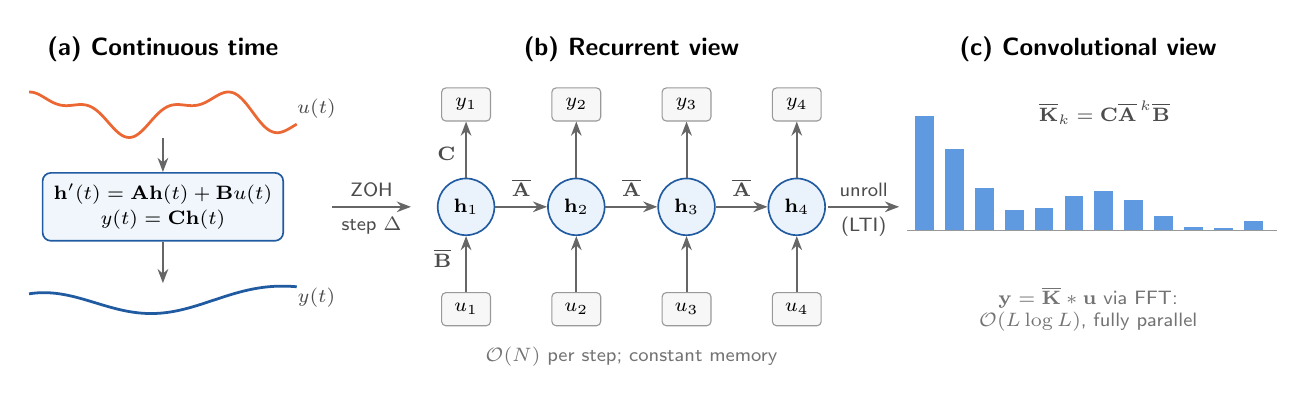
\begin{tikzpicture}[font=\sffamily\scriptsize, arr/.style={-{Stealth[length=1.8mm]}, line width=0.7pt, draw=black!60},
  st/.style={circle, draw=ssm!75!black, fill=ssm!10, line width=0.6pt, minimum size=0.72cm, inner sep=0pt},
  io/.style={rounded corners=1.5pt, draw=black!40, fill=black!3, minimum width=0.62cm, minimum height=0.42cm, inner sep=1pt}]
% (a) continuous
\node[font=\sffamily\bfseries\small] at (2.0,2.55) {(a) Continuous time};
\draw[attn, line width=1pt] plot[smooth, domain=0.3:3.7, samples=60] (\x, {1.75+0.22*sin(deg(3*\x))+0.1*sin(deg(7*\x))});
\node[text=black!70] at (3.95,1.8) {$u(t)$};
\node[draw=ssm!75!black, fill=ssm!7, rounded corners=3pt, align=center, line width=0.6pt, inner sep=4pt] (ode) at (2.0,0.55) {$\vh'(t)=\mA\vh(t)+\mB u(t)$\\[1pt] $y(t)=\mC\vh(t)$};
\draw[arr] (2.0,1.42) -- (ode.north);
\draw[ssm!75!black, line width=1pt] plot[smooth, domain=0.3:3.7, samples=60] (\x, {-0.75+0.2*sin(deg(2.1*\x+0.6))*exp(-0.15*\x)+0.05*\x});
\draw[arr] (ode.south) -- (2.0,-0.42);
\node[text=black!70] at (3.95,-0.6) {$y(t)$};
% arrow a->b
\draw[arr] (4.15,0.55) -- node[above, align=center, text=black!70]{ZOH} node[below, text=black!70]{step $\Delta$} (5.15,0.55);
% (b) recurrent
\node[font=\sffamily\bfseries\small] at (7.95,2.55) {(b) Recurrent view};
\foreach \i/\lab in {0/1,1/2,2/3,3/4} {
  \node[st] (h\i) at (5.85+1.4*\i,0.55) {$\vh_{\lab}$};
  \node[io] (u\i) at (5.85+1.4*\i,-0.75) {$u_{\lab}$};
  \node[io] (y\i) at (5.85+1.4*\i,1.85) {$y_{\lab}$};
  \draw[arr] (u\i) -- (h\i);
  \draw[arr] (h\i) -- (y\i);
}
\foreach \i/\j in {0/1,1/2,2/3} { \draw[arr] (h\i) -- node[above, text=black!70]{$\Ab$} (h\j); }
\node[text=black!70] at (5.55,-0.1) {$\Bb$};
\node[text=black!70] at (5.6,1.22) {$\mC$};
\node[text=black!55, align=center] at (7.95,-1.35) {$\bigO(N)$ per step; constant memory};
% arrow b->c
\draw[arr] (10.45,0.55) -- node[above, text=black!70]{unroll} node[below, text=black!70]{(LTI)} (11.35,0.55);
% (c) convolution
\node[font=\sffamily\bfseries\small] at (13.75,2.55) {(c) Convolutional view};
\draw[black!40, line width=0.5pt] (11.45,0.25) -- (16.15,0.25);
\fill[ssm!75] (11.55,0.25) rectangle ++(0.24,1.450);
\fill[ssm!75] (11.93,0.25) rectangle ++(0.24,1.037);
\fill[ssm!75] (12.31,0.25) rectangle ++(0.24,0.536);
\fill[ssm!75] (12.69,0.25) rectangle ++(0.24,0.258);
\fill[ssm!75] (13.07,0.25) rectangle ++(0.24,0.283);
\fill[ssm!75] (13.45,0.25) rectangle ++(0.24,0.440);
\fill[ssm!75] (13.83,0.25) rectangle ++(0.24,0.503);
\fill[ssm!75] (14.21,0.25) rectangle ++(0.24,0.387);
\fill[ssm!75] (14.59,0.25) rectangle ++(0.24,0.183);
\fill[ssm!75] (14.97,0.25) rectangle ++(0.24,0.042);
\fill[ssm!75] (15.35,0.25) rectangle ++(0.24,0.036);
\fill[ssm!75] (15.73,0.25) rectangle ++(0.24,0.114);
\node[text=black!70, anchor=west] at (13.0,1.75) {$\Kb_k=\mC\Ab^{\,k}\Bb$};
\node[text=black!55, align=center] at (13.75,-0.75) {$\vy=\Kb*\vu$ via FFT:\\ $\bigO(L\log L)$, fully parallel};
\end{tikzpicture}
\end{adjustbox}
\caption{\label{fig:views}Three equivalent views of a linear time-invariant SSM (our illustration). Discretizing the ODE (a) with step $\Delta$ gives a linear recurrence (b), which decodes in constant memory. Because the parameters do not change over time, unrolling it yields a single convolution kernel $\Kb$ (c), which trains in parallel. Selective models (Section~\ref{sec:gen2}) keep (a) and (b) but lose (c).}
\end{figure}

\subsection{A unified recurrence}
\label{sec:unified}
Eqs.~\eqref{eq:linattn} and \eqref{eq:zoh} instantiate one template. Stacking the $d$ per-channel SSM states as rows of a matrix makes the correspondence exact: the input channel plays the role of the value, $\mB$ the key and $\mC$ the query \citep{dao2024ssd}. We therefore write every model in this survey as
\begin{equation}
\label{eq:unified}
\mS_t=\mathcal{T}_t(\mS_{t-1})+\beta_t\,\vv_t\vk_t\T,\qquad \vo_t=\mS_t\vq_t,
\end{equation}
where $\mathcal{T}_t$ is a linear \emph{transition} acting on the state and $\beta_t$ is a write strength. Table~\ref{tab:unified} lists the transitions used by the main families. Its last column anticipates Section~\ref{sec:gen3}: each update is one step of online gradient descent on an implicit per-token objective $\ell_t(\mS)$. In this sense, the history of the field is a history of choosing $\mathcal{T}_t$ and $\ell_t$.

\begin{table}[!t]
\centering
\caption{Linear-time token mixers as instances of Eq.~\eqref{eq:unified}. A check mark in column \textsf{Sel.}\ denotes input-dependent (selective) transitions. For SSMs, $\vv_t{\leftrightarrow}\vx_t$, $\vk_t{\leftrightarrow}\mB_t$, $\vq_t{\leftrightarrow}\mC_t$; scalar write gates (e.g.\ $\Delta_t$ in Mamba-2, the input gate in mLSTM) are absorbed into $\vv_t$ where inessential. The objective column follows the online-learning reading of Section~\ref{sec:gen3}; $\alpha_t,\gamma\in(0,1)$ are decays.}
\label{tab:unified}
\footnotesize
\renewcommand{\arraystretch}{1.25}
\begin{tabularx}{\textwidth}{@{}>{\raggedright\arraybackslash}p{3.55cm} l l c >{\raggedright\arraybackslash}X@{}}
\toprule
\textbf{Model} & \textbf{Transition} $\mathcal{T}_t(\mS)$ & \textbf{Write} & \textbf{Sel.} & \textbf{Implicit per-token objective} $\ell_t(\mS)$ \\
\midrule
\rowcolor{ssm!6} Linear attention \citep{katharopoulos2020transformers} & $\mS$ & $\vv_t\vk_t\T$ & -- & $-\vv_t\T\mS\vk_t$ (correlation; unbounded) \\
RetNet \citep{sun2023retnet} & $\gamma\,\mS$ & $\vv_t\vk_t\T$ & -- & correlation $+$ fixed decay \\
\rowcolor{ssm!6} S4D, LRU \citep{gu2022s4d,orvieto2023lru} & $\mS\,\Ab$ (diagonal, fixed) & $\vx_t\Bb\T$ & -- & correlation $+$ fixed per-dimension decay \\
Mamba \citep{gu2024mamba} & $\mS\odot\exp(\Delta_t\mA)$ & $(\Delta_t\odot\vx_t)\mB_t\T$ & \checkmark & correlation $+$ input-dependent per-entry decay \\
\rowcolor{ssm!6} GLA \citep{yang2024gla} & $\mS\,\mathrm{diag}(\boldsymbol{\alpha}_t)$ & $\vv_t\vk_t\T$ & \checkmark & correlation $+$ input-dependent per-column decay \\
Mamba-2, mLSTM \citep{dao2024ssd,beck2024xlstm} & $\alpha_t\,\mS$ & $\vv_t\vk_t\T$ & \checkmark & correlation $+$ input-dependent scalar decay \\
\rowcolor{delta!8} DeltaNet \citep{yang2024deltanet} & $\mS(\mI-\beta_t\vk_t\vk_t\T)$ & $\beta_t\vv_t\vk_t\T$ & \checkmark & $\tfrac12\lVert\mS\vk_t-\vv_t\rVert^2$ (regression) \\
\rowcolor{delta!8} Gated DeltaNet \citep{yang2025gated} & $\alpha_t\mS(\mI-\beta_t\vk_t\vk_t\T)$ & $\beta_t\vv_t\vk_t\T$ & \checkmark & regression $+$ input-dependent decay \\
\rowcolor{delta!8} TTT, Titans \citep{sun2024ttt,behrouz2025titans} & gradient step on $\mathbf{W}$ & (nonlinear $f_{\mathbf{W}}$) & \checkmark & $\tfrac12\lVert f_{\mathbf{W}}(\vk_t)-\vv_t\rVert^2$ $+$ momentum, decay \\
\bottomrule
\end{tabularx}
\end{table}

\section{The Evolution of Linear-Time Sequence Models}
\label{sec:evolution}

Fig.~\ref{fig:taxonomy} summarizes our reading of the field's development. Rather than a list of models, we present it as three generations, each defined by the bottleneck it removed from its predecessor.

\begin{figure}[t]
\centering
\begin{adjustbox}{max width=\textwidth}
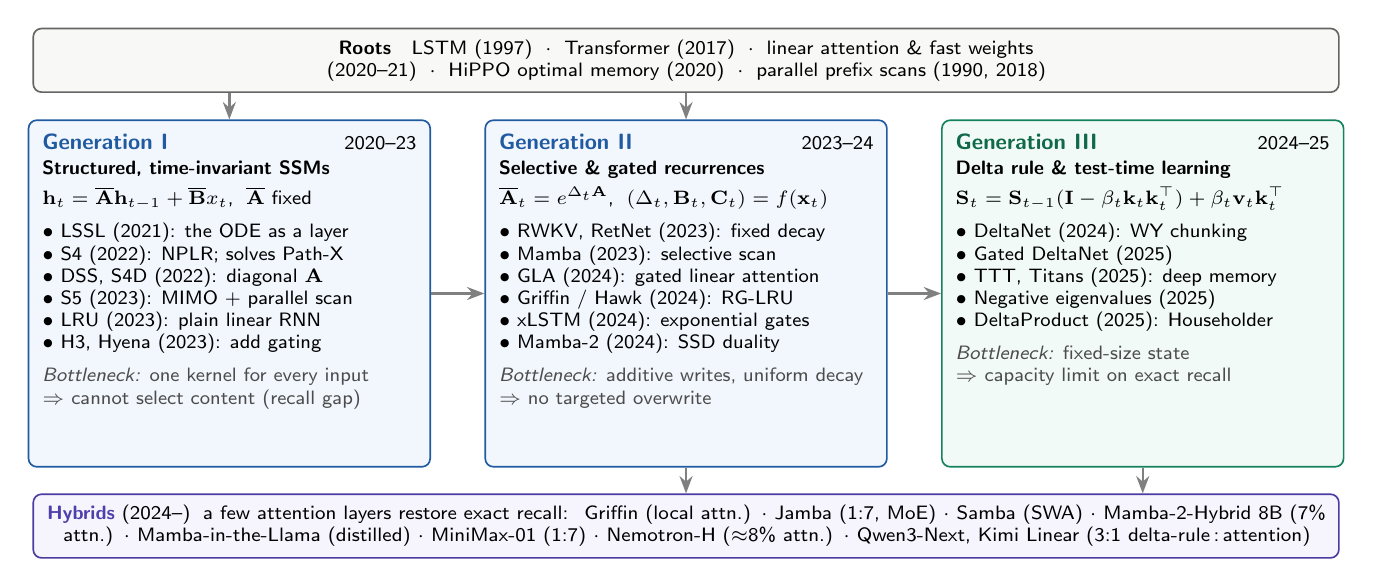
\begin{tikzpicture}[font=\sffamily\scriptsize,
  gen/.style={draw=#1!75!black, fill=#1!6, rounded corners=3pt, line width=0.6pt, inner sep=5pt, anchor=north},
  band/.style={draw=#1!75!black, fill=#1!6, rounded corners=3pt, line width=0.6pt, align=center, text width=16.3cm, inner sep=4pt},
  arr/.style={-{Stealth[length=2.2mm]}, line width=0.9pt, draw=black!50}]
\newcommand{\gbox}[1]{\parbox[t][4.05cm][t]{4.75cm}{\raggedright #1}}
\node[band=muted] (roots) at (8.35,0) {\textbf{Roots}\quad LSTM (1997) \;$\cdot$\; Transformer (2017) \;$\cdot$\; linear attention \& fast weights (2020--21) \;$\cdot$\; HiPPO optimal memory (2020) \;$\cdot$\; parallel prefix scans (1990, 2018)};
\node[gen=ssm] (g1) at (2.55,-0.75) {\gbox{{\footnotesize\textbf{\textcolor{ssm!75!black}{Generation I}}}\hfill 2020--23\\[1pt] \textbf{Structured, time-invariant SSMs}\\[3pt]
$\vh_t=\Ab\vh_{t-1}+\Bb x_t$,\; $\Ab$ fixed\\[4pt]
$\bullet$ LSSL (2021): the ODE as a layer\\
$\bullet$ S4 (2022): NPLR; solves Path-X\\
$\bullet$ DSS, S4D (2022): diagonal $\mA$\\
$\bullet$ S5 (2023): MIMO + parallel scan\\
$\bullet$ LRU (2023): plain linear RNN\\
$\bullet$ H3, Hyena (2023): add gating\\[4pt]
\textcolor{black!70}{\textit{Bottleneck:} one kernel for every input\\ $\Rightarrow$ cannot select content (recall gap)}}};
\node[gen=ssm] (g2) at (8.35,-0.75) {\gbox{{\footnotesize\textbf{\textcolor{ssm!75!black}{Generation II}}}\hfill 2023--24\\[1pt] \textbf{Selective \& gated recurrences}\\[3pt]
$\Ab_t=e^{\Delta_t\mA}$,\; $(\Delta_t,\mB_t,\mC_t)=f(\vx_t)$\\[4pt]
$\bullet$ RWKV, RetNet (2023): fixed decay\\
$\bullet$ Mamba (2023): selective scan\\
$\bullet$ GLA (2024): gated linear attention\\
$\bullet$ Griffin / Hawk (2024): RG-LRU\\
$\bullet$ xLSTM (2024): exponential gates\\
$\bullet$ Mamba-2 (2024): SSD duality\\[4pt]
\textcolor{black!70}{\textit{Bottleneck:} additive writes, uniform decay\\ $\Rightarrow$ no targeted overwrite}}};
\node[gen=delta] (g3) at (14.15,-0.75) {\gbox{{\footnotesize\textbf{\textcolor{delta!60!black}{Generation III}}}\hfill 2024--25\\[1pt] \textbf{Delta rule \& test-time learning}\\[3pt]
$\mS_t=\mS_{t-1}(\mI-\beta_t\vk_t\vk_t\T)+\beta_t\vv_t\vk_t\T$\\[4pt]
$\bullet$ DeltaNet (2024): WY chunking\\
$\bullet$ Gated DeltaNet (2025)\\
$\bullet$ TTT, Titans (2025): deep memory\\
$\bullet$ Negative eigenvalues (2025)\\
$\bullet$ DeltaProduct (2025): Householder\\[4pt]
\textcolor{black!70}{\textit{Bottleneck:} fixed-size state\\ $\Rightarrow$ capacity limit on exact recall}}};
\node[band=hyb, anchor=north] (hy) at (8.35,-5.5) {\textbf{\textcolor{hyb!80!black}{Hybrids}} (2024--)\; a few attention layers restore exact recall:\; Griffin (local attn.) $\cdot$ Jamba (1:7, MoE) $\cdot$ Samba (SWA) $\cdot$ Mamba-2-Hybrid 8B (7\% attn.) $\cdot$ Mamba-in-the-Llama (distilled) $\cdot$ MiniMax-01 (1:7) $\cdot$ Nemotron-H ($\approx$8\% attn.) $\cdot$ Qwen3-Next, Kimi Linear (3:1 delta-rule\,:\,attention)};
\draw[arr] (g1.east) -- (g2.west);
\draw[arr] (g2.east) -- (g3.west);
\draw[arr] (roots.south -| g1.north) -- (g1.north);
\draw[arr] (roots.south -| g2.north) -- (g2.north);
\draw[arr] (g2.south) -- (g2.south |- hy.north);
\draw[arr] (g3.south) -- (g3.south |- hy.north);
\end{tikzpicture}
\end{adjustbox}
\caption{\label{fig:taxonomy}Evolution of linear-time sequence models, organized by the bottleneck each generation removed (our own synthesis; years are first public appearance). Each generation is an instance of Eq.~\eqref{eq:unified} with a richer transition or write rule; hybrids combine Generation II/III layers with a minority of attention layers.}
\end{figure}

\subsection{Generation I: structured, time-invariant state space models}
\label{sec:gen1}
\paragraph{Principled memory.} HiPPO \citep{gu2020hippo} asked what an optimal fixed-size summary of a growing history looks like. Projecting the history $u(s),\,s\le t$, onto the first $N$ Legendre polynomials under a uniform measure yields coefficients $\vh(t)\in\R^N$ that evolve according to a linear ODE of the form of Eq.~\eqref{eq:ssm}, with a specific lower-triangular $\mA$. LSSL \citep{gu2021lssl} embedded this ODE as a deep-learning layer and showed that it subsumes convolutions and (linear) RNNs. Computing the kernel $\Kb$ of Eq.~\eqref{eq:conv} naively, however, requires $L$ successive powers of a dense $N\times N$ matrix, which is slow and numerically unstable.

\paragraph{Making it efficient: S4 and its diagonal descendants.} S4 \citep{gu2022s4} reparameterized the HiPPO matrix as normal plus low-rank, reducing the kernel computation to a well-conditioned Cauchy-kernel evaluation. The result was a qualitative jump on long-range benchmarks: an LRA average of 80.48\% and 88.10\% on Path-X, a task on which every previously reported model either failed or was infeasible \citep{tay2021lra}. A sequence of simplifications followed. DSS \citep{gupta2022dss} found that a purely diagonal $\mA$ performs comparably, and S4D \citep{gu2022s4d} explained why and supplied simple initializations such as S4D-Real, $\lambda_n=-(n+1)$. With diagonal $\mA$, $\Ab$ is diagonal and the kernel becomes a sum of damped (complex) exponentials, $\Kb_k=\sum_{n}C_n\Bb_n e^{k\Delta\lambda_n}$, which a Vandermonde product evaluates cheaply. S5 \citep{smith2023s5} used a single multi-input multi-output diagonal SSM computed with a \emph{parallel scan} instead of a convolution, foreshadowing Generation~II. Finally, the LRU \citep{orvieto2023lru} showed that the continuous-time derivation is not essential: a plain linear RNN with diagonal complex recurrence, a stable exponential parameterization of eigenvalues near the unit circle and input normalization matches S4 on LRA.

\paragraph{Assessment.} Generation~I established the three ingredients still used today: linear recurrences (which can be parallelized), diagonal structure (which makes them cheap), and eigenvalues initialized near $|\lambda|=1$ (which gives long memory). We read the LRU result as demoting the ODE from a source of power to an excellent \emph{parameterization and initialization} device. The decisive limitation is time-invariance. The same kernel $\Kb$ filters every input regardless of content. This suits audio and other continuous signals, where content-independent filtering is natural, but language requires content-dependent routing: \emph{store this name, skip that filler}.

\subsection{Language modeling exposes the recall gap}
\label{sec:gap}
Attempts to apply Generation~I models to language made this limitation concrete. H3 \citep{fu2023h3} found that SSMs struggled on synthetic recall and token-comparison tasks and added multiplicative interactions between projections of the input (a shift SSM, a diagonal SSM and gating). Their hybrid with two attention layers outperformed a Transformer in perplexity. Hyena \citep{poli2023hyena} replaced SSM kernels with implicitly parameterized long convolutions interleaved with data-controlled gating. RWKV \citep{peng2023rwkv} and RetNet \citep{sun2023retnet} derived recurrences with fixed exponential decays from linear attention and scaled them to billions of parameters with parallel training and $\bigO(1)$ decoding. Zoology \citep{arora2024zoology} supplied the diagnosis. On the Pile, 82\% of the perplexity gap between gated-convolution models and attention is explained by \emph{associative recall}, and on a multi-query associative recall (MQAR) task a 70M-parameter attention model outperforms a 1.4B-parameter gated-convolution model. The missing ingredient was not capacity per se but \emph{input-dependent selection} of what to write and what to keep.

\subsection{Generation II: selectivity and data-dependent gating}
\label{sec:gen2}
\paragraph{Selective SSMs.} Mamba \citep{gu2024mamba} makes the step size and the input and output matrices functions of the current token, using a real diagonal $\mA$ (S4D-Real initialization) and state size $N{=}16$:
\begin{equation}
\label{eq:selective}
\Delta_t=\softplus(\mathbf{w}_\Delta\T\vx_t+b_\Delta),\quad \mB_t=\mathbf{W}_B\vx_t,\quad \mC_t=\mathbf{W}_C\vx_t,\qquad \vh_t=e^{\Delta_t\mA}\vh_{t-1}+\Bb_t x_t,\quad y_t=\mC_t\T\vh_t,
\end{equation}
with $\Bb_t=\mA^{-1}(e^{\Delta_t\mA}-\mI)\mB_t\approx\Delta_t\mB_t$ for small $\Delta_t$. The step $\Delta_t$ acts as a content-dependent clock. As $\Delta_t\to0$, $e^{\Delta_t\mA}\to\mI$ and $\Bb_t\to\mathbf{0}$: the token is ignored and the state is preserved. As $\Delta_t\to\infty$, $e^{\Delta_t\mA}\to\mathbf{0}$ (since $\lambda(\mA)<0$): the state is reset and the token dominates. Selectivity is a principled form of classical gating. With $N=1$, $\mA=-1$ and $\mB=1$, the ZOH formulas give $\Ab_t=e^{-\Delta_t}$ and $\Bb_t=1-e^{-\Delta_t}$. Writing $\Delta_t=\softplus(z_t)=\log(1+e^{z_t})$,
\begin{equation}
\label{eq:gate}
1-e^{-\Delta_t}=1-\frac{1}{1+e^{z_t}}=\sigma(z_t)\quad\Longrightarrow\quad h_t=\big(1-\sigma(z_t)\big)\,h_{t-1}+\sigma(z_t)\,x_t ,
\end{equation}
which is exactly a gated leaky-integrator RNN \citep[Thm.~1]{gu2024mamba}.

\paragraph{The price of selectivity, and the scan.} Input-dependent $\Ab_t$ destroys the convolution view, because there is no longer a single kernel. Mamba instead evaluates the recurrence with a parallel scan. Each step is an affine map $h\mapsto a_th+b_t$, and composing two such maps yields another affine map:
\begin{equation}
\label{eq:scan}
(a_1,b_1)\bullet(a_2,b_2)=(a_2a_1,\ a_2b_1+b_2).
\end{equation}
The operator $\bullet$ is associative, so all prefixes $h_1,\dots,h_L$ can be computed with $\bigO(L)$ work and $\bigO(\log L)$ depth \citep{blelloch1990prefix,martin2018parallelizing}. Mamba's kernel fuses discretization, scan and readout in on-chip SRAM, never materializing the $(L\times d\times N)$ expanded state in high-bandwidth memory, and recomputes it in the backward pass. The result is $5\times$ higher inference throughput than Transformers, and a 3B model that matches Transformers twice its size in pretraining and downstream evaluation \citep{gu2024mamba}.

\paragraph{Gated linear attention and gated RNNs.} Contemporaneous work reached the same idea from the attention side. GLA \citep{yang2024gla} adds a data-dependent diagonal gate to matrix-valued linear attention and introduces a chunkwise, tensor-core-friendly training algorithm. Griffin \citep{de2024griffin} introduces the real-gated linear recurrent unit (RG-LRU) and mixes it with local attention (window 1024); the hybrid matches Llama-2 while training on over $6\times$ fewer tokens. xLSTM \citep{beck2024xlstm} revisits the LSTM with exponential gating and a matrix memory (mLSTM) that is again an instance of Eq.~\eqref{eq:unified}.

\subsection{Structured state space duality}
\label{sec:ssd}
Mamba-2 \citep{dao2024ssd} restricts the transition to a scalar per head, $\Ab_t=a_t\mI$. Unrolling the recurrence then gives
\begin{equation}
\label{eq:ssd}
y_t=\sum_{s\le t}\mC_t\T\Big(\prod_{r=s+1}^{t}a_r\Big)\mB_s\,x_s
\quad\Longleftrightarrow\quad
\vy=\big(\mL\circ\mC\mB\T\big)\,\vx,\qquad
\mL_{ts}=\begin{cases}\prod_{r=s+1}^{t}a_r=\Lambda_t/\Lambda_s,& t\ge s,\\ 0,& t<s,\end{cases}
\end{equation}
where $\Lambda_t=\prod_{r\le t}a_r$. With $a_r\equiv1$, $\mL$ is the causal mask and Eq.~\eqref{eq:ssd} is exactly causal linear attention with queries $\mC$, keys $\mB$ and values $\vx$. Because $\mL_{ts}=\Lambda_t\Lambda_s^{-1}$, every block of $\mL$ strictly below the diagonal has rank one: $\mL$ is \emph{1-semiseparable}. This yields a chunkwise algorithm (Fig.~\ref{fig:masks}). Diagonal blocks of size $Q$ are computed in the quadratic, attention-like form with dense matrix multiplications, and off-diagonal blocks are routed through the recurrent state between chunks. The core layer is 2--8$\times$ faster than Mamba's scan and admits states 8$\times$ larger or more (typically $N{=}64$ or $128$).

\begin{figure}[t]
\centering
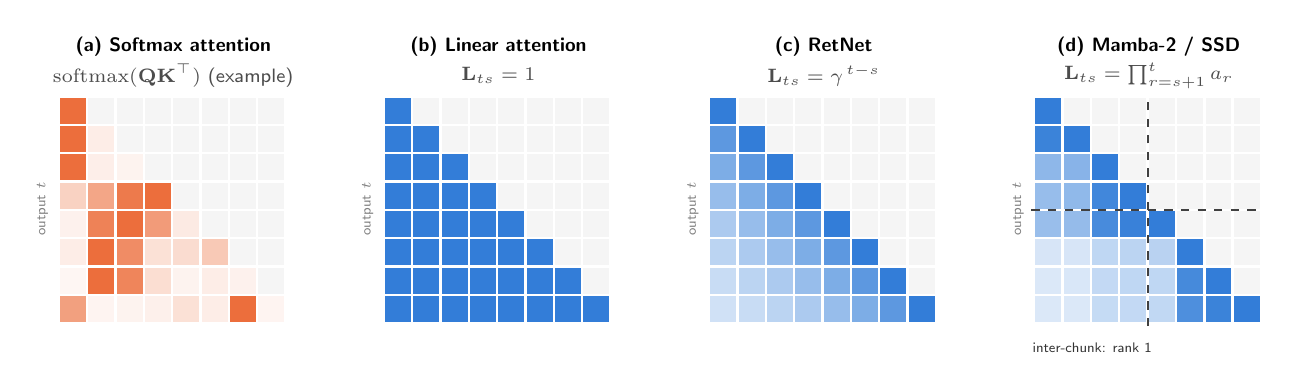
\begin{tikzpicture}
\node[font=\sffamily\bfseries\scriptsize, align=center] at (1.44,3.50) {(a) Softmax attention};
\node[font=\sffamily\scriptsize, text=black!70] at (1.44,3.13) {$\mathrm{softmax}(\mathbf{QK}\T)$ (example)};
\fill[attn!96!white] (0.000,2.520) rectangle ++(0.33,0.33);
\fill[black!4] (0.360,2.520) rectangle ++(0.33,0.33);
\fill[black!4] (0.720,2.520) rectangle ++(0.33,0.33);
\fill[black!4] (1.080,2.520) rectangle ++(0.33,0.33);
\fill[black!4] (1.440,2.520) rectangle ++(0.33,0.33);
\fill[black!4] (1.800,2.520) rectangle ++(0.33,0.33);
\fill[black!4] (2.160,2.520) rectangle ++(0.33,0.33);
\fill[black!4] (2.520,2.520) rectangle ++(0.33,0.33);
\fill[attn!96!white] (0.000,2.160) rectangle ++(0.33,0.33);
\fill[attn!12!white] (0.360,2.160) rectangle ++(0.33,0.33);
\fill[black!4] (0.720,2.160) rectangle ++(0.33,0.33);
\fill[black!4] (1.080,2.160) rectangle ++(0.33,0.33);
\fill[black!4] (1.440,2.160) rectangle ++(0.33,0.33);
\fill[black!4] (1.800,2.160) rectangle ++(0.33,0.33);
\fill[black!4] (2.160,2.160) rectangle ++(0.33,0.33);
\fill[black!4] (2.520,2.160) rectangle ++(0.33,0.33);
\fill[attn!96!white] (0.000,1.800) rectangle ++(0.33,0.33);
\fill[attn!11!white] (0.360,1.800) rectangle ++(0.33,0.33);
\fill[attn!8!white] (0.720,1.800) rectangle ++(0.33,0.33);
\fill[black!4] (1.080,1.800) rectangle ++(0.33,0.33);
\fill[black!4] (1.440,1.800) rectangle ++(0.33,0.33);
\fill[black!4] (1.800,1.800) rectangle ++(0.33,0.33);
\fill[black!4] (2.160,1.800) rectangle ++(0.33,0.33);
\fill[black!4] (2.520,1.800) rectangle ++(0.33,0.33);
\fill[attn!30!white] (0.000,1.440) rectangle ++(0.33,0.33);
\fill[attn!59!white] (0.360,1.440) rectangle ++(0.33,0.33);
\fill[attn!88!white] (0.720,1.440) rectangle ++(0.33,0.33);
\fill[attn!96!white] (1.080,1.440) rectangle ++(0.33,0.33);
\fill[black!4] (1.440,1.440) rectangle ++(0.33,0.33);
\fill[black!4] (1.800,1.440) rectangle ++(0.33,0.33);
\fill[black!4] (2.160,1.440) rectangle ++(0.33,0.33);
\fill[black!4] (2.520,1.440) rectangle ++(0.33,0.33);
\fill[attn!9!white] (0.000,1.080) rectangle ++(0.33,0.33);
\fill[attn!83!white] (0.360,1.080) rectangle ++(0.33,0.33);
\fill[attn!96!white] (0.720,1.080) rectangle ++(0.33,0.33);
\fill[attn!66!white] (1.080,1.080) rectangle ++(0.33,0.33);
\fill[attn!14!white] (1.440,1.080) rectangle ++(0.33,0.33);
\fill[black!4] (1.800,1.080) rectangle ++(0.33,0.33);
\fill[black!4] (2.160,1.080) rectangle ++(0.33,0.33);
\fill[black!4] (2.520,1.080) rectangle ++(0.33,0.33);
\fill[attn!12!white] (0.000,0.720) rectangle ++(0.33,0.33);
\fill[attn!96!white] (0.360,0.720) rectangle ++(0.33,0.33);
\fill[attn!76!white] (0.720,0.720) rectangle ++(0.33,0.33);
\fill[attn!20!white] (1.080,0.720) rectangle ++(0.33,0.33);
\fill[attn!23!white] (1.440,0.720) rectangle ++(0.33,0.33);
\fill[attn!36!white] (1.800,0.720) rectangle ++(0.33,0.33);
\fill[black!4] (2.160,0.720) rectangle ++(0.33,0.33);
\fill[black!4] (2.520,0.720) rectangle ++(0.33,0.33);
\fill[attn!6!white] (0.000,0.360) rectangle ++(0.33,0.33);
\fill[attn!96!white] (0.360,0.360) rectangle ++(0.33,0.33);
\fill[attn!81!white] (0.720,0.360) rectangle ++(0.33,0.33);
\fill[attn!22!white] (1.080,0.360) rectangle ++(0.33,0.33);
\fill[attn!8!white] (1.440,0.360) rectangle ++(0.33,0.33);
\fill[attn!12!white] (1.800,0.360) rectangle ++(0.33,0.33);
\fill[attn!9!white] (2.160,0.360) rectangle ++(0.33,0.33);
\fill[black!4] (2.520,0.360) rectangle ++(0.33,0.33);
\fill[attn!63!white] (0.000,0.000) rectangle ++(0.33,0.33);
\fill[attn!7!white] (0.360,0.000) rectangle ++(0.33,0.33);
\fill[attn!8!white] (0.720,0.000) rectangle ++(0.33,0.33);
\fill[attn!10!white] (1.080,0.000) rectangle ++(0.33,0.33);
\fill[attn!20!white] (1.440,0.000) rectangle ++(0.33,0.33);
\fill[attn!12!white] (1.800,0.000) rectangle ++(0.33,0.33);
\fill[attn!96!white] (2.160,0.000) rectangle ++(0.33,0.33);
\fill[attn!7!white] (2.520,0.000) rectangle ++(0.33,0.33);
\node[font=\sffamily\tiny, text=black!50, rotate=90] at (-0.22,1.44) {output $t$};
\node[font=\sffamily\bfseries\scriptsize, align=center] at (5.57,3.50) {(b) Linear attention};
\node[font=\sffamily\scriptsize, text=black!70] at (5.57,3.13) {$\mL_{ts}=1$};
\fill[ssm!96!white] (4.130,2.520) rectangle ++(0.33,0.33);
\fill[black!4] (4.490,2.520) rectangle ++(0.33,0.33);
\fill[black!4] (4.850,2.520) rectangle ++(0.33,0.33);
\fill[black!4] (5.210,2.520) rectangle ++(0.33,0.33);
\fill[black!4] (5.570,2.520) rectangle ++(0.33,0.33);
\fill[black!4] (5.930,2.520) rectangle ++(0.33,0.33);
\fill[black!4] (6.290,2.520) rectangle ++(0.33,0.33);
\fill[black!4] (6.650,2.520) rectangle ++(0.33,0.33);
\fill[ssm!96!white] (4.130,2.160) rectangle ++(0.33,0.33);
\fill[ssm!96!white] (4.490,2.160) rectangle ++(0.33,0.33);
\fill[black!4] (4.850,2.160) rectangle ++(0.33,0.33);
\fill[black!4] (5.210,2.160) rectangle ++(0.33,0.33);
\fill[black!4] (5.570,2.160) rectangle ++(0.33,0.33);
\fill[black!4] (5.930,2.160) rectangle ++(0.33,0.33);
\fill[black!4] (6.290,2.160) rectangle ++(0.33,0.33);
\fill[black!4] (6.650,2.160) rectangle ++(0.33,0.33);
\fill[ssm!96!white] (4.130,1.800) rectangle ++(0.33,0.33);
\fill[ssm!96!white] (4.490,1.800) rectangle ++(0.33,0.33);
\fill[ssm!96!white] (4.850,1.800) rectangle ++(0.33,0.33);
\fill[black!4] (5.210,1.800) rectangle ++(0.33,0.33);
\fill[black!4] (5.570,1.800) rectangle ++(0.33,0.33);
\fill[black!4] (5.930,1.800) rectangle ++(0.33,0.33);
\fill[black!4] (6.290,1.800) rectangle ++(0.33,0.33);
\fill[black!4] (6.650,1.800) rectangle ++(0.33,0.33);
\fill[ssm!96!white] (4.130,1.440) rectangle ++(0.33,0.33);
\fill[ssm!96!white] (4.490,1.440) rectangle ++(0.33,0.33);
\fill[ssm!96!white] (4.850,1.440) rectangle ++(0.33,0.33);
\fill[ssm!96!white] (5.210,1.440) rectangle ++(0.33,0.33);
\fill[black!4] (5.570,1.440) rectangle ++(0.33,0.33);
\fill[black!4] (5.930,1.440) rectangle ++(0.33,0.33);
\fill[black!4] (6.290,1.440) rectangle ++(0.33,0.33);
\fill[black!4] (6.650,1.440) rectangle ++(0.33,0.33);
\fill[ssm!96!white] (4.130,1.080) rectangle ++(0.33,0.33);
\fill[ssm!96!white] (4.490,1.080) rectangle ++(0.33,0.33);
\fill[ssm!96!white] (4.850,1.080) rectangle ++(0.33,0.33);
\fill[ssm!96!white] (5.210,1.080) rectangle ++(0.33,0.33);
\fill[ssm!96!white] (5.570,1.080) rectangle ++(0.33,0.33);
\fill[black!4] (5.930,1.080) rectangle ++(0.33,0.33);
\fill[black!4] (6.290,1.080) rectangle ++(0.33,0.33);
\fill[black!4] (6.650,1.080) rectangle ++(0.33,0.33);
\fill[ssm!96!white] (4.130,0.720) rectangle ++(0.33,0.33);
\fill[ssm!96!white] (4.490,0.720) rectangle ++(0.33,0.33);
\fill[ssm!96!white] (4.850,0.720) rectangle ++(0.33,0.33);
\fill[ssm!96!white] (5.210,0.720) rectangle ++(0.33,0.33);
\fill[ssm!96!white] (5.570,0.720) rectangle ++(0.33,0.33);
\fill[ssm!96!white] (5.930,0.720) rectangle ++(0.33,0.33);
\fill[black!4] (6.290,0.720) rectangle ++(0.33,0.33);
\fill[black!4] (6.650,0.720) rectangle ++(0.33,0.33);
\fill[ssm!96!white] (4.130,0.360) rectangle ++(0.33,0.33);
\fill[ssm!96!white] (4.490,0.360) rectangle ++(0.33,0.33);
\fill[ssm!96!white] (4.850,0.360) rectangle ++(0.33,0.33);
\fill[ssm!96!white] (5.210,0.360) rectangle ++(0.33,0.33);
\fill[ssm!96!white] (5.570,0.360) rectangle ++(0.33,0.33);
\fill[ssm!96!white] (5.930,0.360) rectangle ++(0.33,0.33);
\fill[ssm!96!white] (6.290,0.360) rectangle ++(0.33,0.33);
\fill[black!4] (6.650,0.360) rectangle ++(0.33,0.33);
\fill[ssm!96!white] (4.130,0.000) rectangle ++(0.33,0.33);
\fill[ssm!96!white] (4.490,0.000) rectangle ++(0.33,0.33);
\fill[ssm!96!white] (4.850,0.000) rectangle ++(0.33,0.33);
\fill[ssm!96!white] (5.210,0.000) rectangle ++(0.33,0.33);
\fill[ssm!96!white] (5.570,0.000) rectangle ++(0.33,0.33);
\fill[ssm!96!white] (5.930,0.000) rectangle ++(0.33,0.33);
\fill[ssm!96!white] (6.290,0.000) rectangle ++(0.33,0.33);
\fill[ssm!96!white] (6.650,0.000) rectangle ++(0.33,0.33);
\node[font=\sffamily\tiny, text=black!50, rotate=90] at (3.91,1.44) {output $t$};
\node[font=\sffamily\bfseries\scriptsize, align=center] at (9.70,3.50) {(c) RetNet};
\node[font=\sffamily\scriptsize, text=black!70] at (9.70,3.13) {$\mL_{ts}=\gamma^{\,t-s}$};
\fill[ssm!96!white] (8.260,2.520) rectangle ++(0.33,0.33);
\fill[black!4] (8.620,2.520) rectangle ++(0.33,0.33);
\fill[black!4] (8.980,2.520) rectangle ++(0.33,0.33);
\fill[black!4] (9.340,2.520) rectangle ++(0.33,0.33);
\fill[black!4] (9.700,2.520) rectangle ++(0.33,0.33);
\fill[black!4] (10.060,2.520) rectangle ++(0.33,0.33);
\fill[black!4] (10.420,2.520) rectangle ++(0.33,0.33);
\fill[black!4] (10.780,2.520) rectangle ++(0.33,0.33);
\fill[ssm!76!white] (8.260,2.160) rectangle ++(0.33,0.33);
\fill[ssm!96!white] (8.620,2.160) rectangle ++(0.33,0.33);
\fill[black!4] (8.980,2.160) rectangle ++(0.33,0.33);
\fill[black!4] (9.340,2.160) rectangle ++(0.33,0.33);
\fill[black!4] (9.700,2.160) rectangle ++(0.33,0.33);
\fill[black!4] (10.060,2.160) rectangle ++(0.33,0.33);
\fill[black!4] (10.420,2.160) rectangle ++(0.33,0.33);
\fill[black!4] (10.780,2.160) rectangle ++(0.33,0.33);
\fill[ssm!61!white] (8.260,1.800) rectangle ++(0.33,0.33);
\fill[ssm!76!white] (8.620,1.800) rectangle ++(0.33,0.33);
\fill[ssm!96!white] (8.980,1.800) rectangle ++(0.33,0.33);
\fill[black!4] (9.340,1.800) rectangle ++(0.33,0.33);
\fill[black!4] (9.700,1.800) rectangle ++(0.33,0.33);
\fill[black!4] (10.060,1.800) rectangle ++(0.33,0.33);
\fill[black!4] (10.420,1.800) rectangle ++(0.33,0.33);
\fill[black!4] (10.780,1.800) rectangle ++(0.33,0.33);
\fill[ssm!49!white] (8.260,1.440) rectangle ++(0.33,0.33);
\fill[ssm!61!white] (8.620,1.440) rectangle ++(0.33,0.33);
\fill[ssm!76!white] (8.980,1.440) rectangle ++(0.33,0.33);
\fill[ssm!96!white] (9.340,1.440) rectangle ++(0.33,0.33);
\fill[black!4] (9.700,1.440) rectangle ++(0.33,0.33);
\fill[black!4] (10.060,1.440) rectangle ++(0.33,0.33);
\fill[black!4] (10.420,1.440) rectangle ++(0.33,0.33);
\fill[black!4] (10.780,1.440) rectangle ++(0.33,0.33);
\fill[ssm!39!white] (8.260,1.080) rectangle ++(0.33,0.33);
\fill[ssm!49!white] (8.620,1.080) rectangle ++(0.33,0.33);
\fill[ssm!61!white] (8.980,1.080) rectangle ++(0.33,0.33);
\fill[ssm!76!white] (9.340,1.080) rectangle ++(0.33,0.33);
\fill[ssm!96!white] (9.700,1.080) rectangle ++(0.33,0.33);
\fill[black!4] (10.060,1.080) rectangle ++(0.33,0.33);
\fill[black!4] (10.420,1.080) rectangle ++(0.33,0.33);
\fill[black!4] (10.780,1.080) rectangle ++(0.33,0.33);
\fill[ssm!32!white] (8.260,0.720) rectangle ++(0.33,0.33);
\fill[ssm!39!white] (8.620,0.720) rectangle ++(0.33,0.33);
\fill[ssm!49!white] (8.980,0.720) rectangle ++(0.33,0.33);
\fill[ssm!61!white] (9.340,0.720) rectangle ++(0.33,0.33);
\fill[ssm!76!white] (9.700,0.720) rectangle ++(0.33,0.33);
\fill[ssm!96!white] (10.060,0.720) rectangle ++(0.33,0.33);
\fill[black!4] (10.420,0.720) rectangle ++(0.33,0.33);
\fill[black!4] (10.780,0.720) rectangle ++(0.33,0.33);
\fill[ssm!26!white] (8.260,0.360) rectangle ++(0.33,0.33);
\fill[ssm!32!white] (8.620,0.360) rectangle ++(0.33,0.33);
\fill[ssm!39!white] (8.980,0.360) rectangle ++(0.33,0.33);
\fill[ssm!49!white] (9.340,0.360) rectangle ++(0.33,0.33);
\fill[ssm!61!white] (9.700,0.360) rectangle ++(0.33,0.33);
\fill[ssm!76!white] (10.060,0.360) rectangle ++(0.33,0.33);
\fill[ssm!96!white] (10.420,0.360) rectangle ++(0.33,0.33);
\fill[black!4] (10.780,0.360) rectangle ++(0.33,0.33);
\fill[ssm!22!white] (8.260,0.000) rectangle ++(0.33,0.33);
\fill[ssm!26!white] (8.620,0.000) rectangle ++(0.33,0.33);
\fill[ssm!32!white] (8.980,0.000) rectangle ++(0.33,0.33);
\fill[ssm!39!white] (9.340,0.000) rectangle ++(0.33,0.33);
\fill[ssm!49!white] (9.700,0.000) rectangle ++(0.33,0.33);
\fill[ssm!61!white] (10.060,0.000) rectangle ++(0.33,0.33);
\fill[ssm!76!white] (10.420,0.000) rectangle ++(0.33,0.33);
\fill[ssm!96!white] (10.780,0.000) rectangle ++(0.33,0.33);
\node[font=\sffamily\tiny, text=black!50, rotate=90] at (8.04,1.44) {output $t$};
\node[font=\sffamily\bfseries\scriptsize, align=center] at (13.83,3.50) {(d) Mamba-2 / SSD};
\node[font=\sffamily\scriptsize, text=black!70] at (13.83,3.13) {$\mL_{ts}=\prod_{r=s+1}^{t}a_r$};
\fill[ssm!96!white] (12.390,2.520) rectangle ++(0.33,0.33);
\fill[black!4] (12.750,2.520) rectangle ++(0.33,0.33);
\fill[black!4] (13.110,2.520) rectangle ++(0.33,0.33);
\fill[black!4] (13.470,2.520) rectangle ++(0.33,0.33);
\fill[black!4] (13.830,2.520) rectangle ++(0.33,0.33);
\fill[black!4] (14.190,2.520) rectangle ++(0.33,0.33);
\fill[black!4] (14.550,2.520) rectangle ++(0.33,0.33);
\fill[black!4] (14.910,2.520) rectangle ++(0.33,0.33);
\fill[ssm!92!white] (12.390,2.160) rectangle ++(0.33,0.33);
\fill[ssm!96!white] (12.750,2.160) rectangle ++(0.33,0.33);
\fill[black!4] (13.110,2.160) rectangle ++(0.33,0.33);
\fill[black!4] (13.470,2.160) rectangle ++(0.33,0.33);
\fill[black!4] (13.830,2.160) rectangle ++(0.33,0.33);
\fill[black!4] (14.190,2.160) rectangle ++(0.33,0.33);
\fill[black!4] (14.550,2.160) rectangle ++(0.33,0.33);
\fill[black!4] (14.910,2.160) rectangle ++(0.33,0.33);
\fill[ssm!53!white] (12.390,1.800) rectangle ++(0.33,0.33);
\fill[ssm!56!white] (12.750,1.800) rectangle ++(0.33,0.33);
\fill[ssm!96!white] (13.110,1.800) rectangle ++(0.33,0.33);
\fill[black!4] (13.470,1.800) rectangle ++(0.33,0.33);
\fill[black!4] (13.830,1.800) rectangle ++(0.33,0.33);
\fill[black!4] (14.190,1.800) rectangle ++(0.33,0.33);
\fill[black!4] (14.550,1.800) rectangle ++(0.33,0.33);
\fill[black!4] (14.910,1.800) rectangle ++(0.33,0.33);
\fill[ssm!49!white] (12.390,1.440) rectangle ++(0.33,0.33);
\fill[ssm!52!white] (12.750,1.440) rectangle ++(0.33,0.33);
\fill[ssm!89!white] (13.110,1.440) rectangle ++(0.33,0.33);
\fill[ssm!96!white] (13.470,1.440) rectangle ++(0.33,0.33);
\fill[black!4] (13.830,1.440) rectangle ++(0.33,0.33);
\fill[black!4] (14.190,1.440) rectangle ++(0.33,0.33);
\fill[black!4] (14.550,1.440) rectangle ++(0.33,0.33);
\fill[black!4] (14.910,1.440) rectangle ++(0.33,0.33);
\fill[ssm!48!white] (12.390,1.080) rectangle ++(0.33,0.33);
\fill[ssm!50!white] (12.750,1.080) rectangle ++(0.33,0.33);
\fill[ssm!86!white] (13.110,1.080) rectangle ++(0.33,0.33);
\fill[ssm!93!white] (13.470,1.080) rectangle ++(0.33,0.33);
\fill[ssm!96!white] (13.830,1.080) rectangle ++(0.33,0.33);
\fill[black!4] (14.190,1.080) rectangle ++(0.33,0.33);
\fill[black!4] (14.550,1.080) rectangle ++(0.33,0.33);
\fill[black!4] (14.910,1.080) rectangle ++(0.33,0.33);
\fill[ssm!19!white] (12.390,0.720) rectangle ++(0.33,0.33);
\fill[ssm!19!white] (12.750,0.720) rectangle ++(0.33,0.33);
\fill[ssm!30!white] (13.110,0.720) rectangle ++(0.33,0.33);
\fill[ssm!32!white] (13.470,0.720) rectangle ++(0.33,0.33);
\fill[ssm!33!white] (13.830,0.720) rectangle ++(0.33,0.33);
\fill[ssm!96!white] (14.190,0.720) rectangle ++(0.33,0.33);
\fill[black!4] (14.550,0.720) rectangle ++(0.33,0.33);
\fill[black!4] (14.910,0.720) rectangle ++(0.33,0.33);
\fill[ssm!17!white] (12.390,0.360) rectangle ++(0.33,0.33);
\fill[ssm!18!white] (12.750,0.360) rectangle ++(0.33,0.33);
\fill[ssm!28!white] (13.110,0.360) rectangle ++(0.33,0.33);
\fill[ssm!30!white] (13.470,0.360) rectangle ++(0.33,0.33);
\fill[ssm!30!white] (13.830,0.360) rectangle ++(0.33,0.33);
\fill[ssm!87!white] (14.190,0.360) rectangle ++(0.33,0.33);
\fill[ssm!96!white] (14.550,0.360) rectangle ++(0.33,0.33);
\fill[black!4] (14.910,0.360) rectangle ++(0.33,0.33);
\fill[ssm!17!white] (12.390,0.000) rectangle ++(0.33,0.33);
\fill[ssm!17!white] (12.750,0.000) rectangle ++(0.33,0.33);
\fill[ssm!27!white] (13.110,0.000) rectangle ++(0.33,0.33);
\fill[ssm!28!white] (13.470,0.000) rectangle ++(0.33,0.33);
\fill[ssm!29!white] (13.830,0.000) rectangle ++(0.33,0.33);
\fill[ssm!83!white] (14.190,0.000) rectangle ++(0.33,0.33);
\fill[ssm!92!white] (14.550,0.000) rectangle ++(0.33,0.33);
\fill[ssm!96!white] (14.910,0.000) rectangle ++(0.33,0.33);
\draw[black!75, line width=0.8pt, dashed] (13.815,-0.05) -- (13.815,2.88);
\draw[black!75, line width=0.8pt, dashed] (12.34,1.425) -- (15.27,1.425);
\node[font=\sffamily\tiny, text=black!80, align=center] at (13.11,-0.32) {inter-chunk: rank 1};
\node[font=\sffamily\tiny, text=black!50, rotate=90] at (12.17,1.44) {output $t$};
\end{tikzpicture}
\caption{\label{fig:masks}Token-mixing matrices of four families (our computation on toy inputs; darker = larger weight, gray = masked). Softmax attention (a) is dense, data-dependent and row-normalized. Linear-time models multiply $\mathbf{QK}\T$ (or $\mC\mB\T$) by a structured mask $\mL$: all ones for linear attention (b), a fixed Toeplitz decay for RetNet (c), and an input-dependent, 1-semiseparable decay for Mamba-2 (d), where the small $a_3$ and $a_6$ act as \emph{forget} events. Dashed lines in (d) mark chunks of size $Q{=}4$: diagonal blocks are computed as dense matrix multiplications, while off-diagonal blocks have rank one and are passed through the recurrent state.}
\end{figure}

\begin{takeaway}[Takeaway.]
SSD dissolves the \textquotedblleft SSM versus attention\textquotedblright{} dichotomy: both are $\vy=(\mM\circ\mathbf{Q}\mathbf{K}\T)\mathbf{V}$-type operators, differing only in the mask $\mM$ (softmax-normalized and dense, or decaying and semiseparable). It also illustrates a recurring trade-off: the scalar transition of Mamba-2 is strictly \emph{less} expressive than Mamba's per-channel diagonal one, but it maps onto tensor cores and so affords larger states.
\end{takeaway}

\subsection{Generation III: the delta rule and test-time regression}
\label{sec:gen3}
\paragraph{Why additive writes saturate.} Decays forget \emph{uniformly}: $\alpha_t$ shrinks every stored association at once, and no transition in Generation~II can replace the value bound to one particular key. Consider the additive memory $\mS=\sum_i\vv_i\vk_i\T$ with unit-norm keys. Reading with a stored key gives
\begin{equation}
\label{eq:crosstalk}
\mS\vk_j=\vv_j\underbrace{\vk_j\T\vk_j}_{=1}+\sum_{i\neq j}\vv_i\,(\vk_i\T\vk_j),
\end{equation}
the target plus a crosstalk term that vanishes only if the keys are orthogonal, which is impossible for more than $d_k$ of them.

\paragraph{The delta rule as one step of online regression.} Treat the state as a linear regressor that should map $\vk_t$ to $\vv_t$, and take one gradient step on $\ell_t(\mS)=\tfrac12\lVert\mS\vk_t-\vv_t\rVert^2$. Since $\nabla_{\mS}\ell_t=(\mS\vk_t-\vv_t)\vk_t\T$,
\begin{equation}
\label{eq:delta}
\mS_t=\mS_{t-1}-\beta_t(\mS_{t-1}\vk_t-\vv_t)\vk_t\T=\mS_{t-1}\big(\mI-\beta_t\vk_t\vk_t\T\big)+\beta_t\vv_t\vk_t\T .
\end{equation}
For a unit key, $\mS_t\vk_t=(1-\beta_t)\mS_{t-1}\vk_t+\beta_t\vv_t$, so $\beta_t=1$ \emph{overwrites} the old association exactly. The same reading recovers linear attention as one gradient step on $\ell_t(\mS)=-\vv_t\T\mS\vk_t$, whose gradient is $-\vv_t\vk_t\T$. That objective rewards correlation and has no error-correcting term. The delta rule dates back to Widrow--Hoff and was proposed for linear Transformers by \citet{schlag2021linear}; \citet{yang2024deltanet} made it practical. The transition $\mI-\beta_t\vk_t\vk_t\T$ is a generalized Householder matrix, and products of such matrices admit a compact WY representation. This enables chunkwise parallel training on tensor cores and scaling DeltaNet to 1.3B parameters, where it outperforms Mamba and GLA in perplexity and zero-shot downstream performance.

\paragraph{Gating plus delta.} Gated DeltaNet \citep{yang2025gated} combines the two mechanisms, $\mS_t=\alpha_t\mS_{t-1}(\mI-\beta_t\vk_t\vk_t\T)+\beta_t\vv_t\vk_t\T$. This is a decay step (input-dependent weight decay) followed by a delta step. The gate allows rapid global erasure and the delta rule targeted overwrites, and the combination surpasses both Mamba-2 and DeltaNet in language modeling, in-context retrieval, length extrapolation and long-context understanding.

\paragraph{Learning at test time.} If the state is a regressor trained online, nothing forces it to be linear or the optimizer to be plain gradient descent. TTT layers \citep{sun2024ttt} make the hidden state the weights $\mathbf{W}$ of a linear model or an MLP, updated by gradient steps on a self-supervised reconstruction loss. TTT-Linear is closely related to Eq.~\eqref{eq:delta}. Titans \citep{behrouz2025titans} use a deep MLP memory updated with momentum (\textquotedblleft surprise\textquotedblright) and weight decay (forgetting), alongside attention as short-term memory. \citet{wang2025testtimeregression} formalize the design space as a choice of regression objective, memory function class and optimizer, and recover most of Table~\ref{tab:unified} as special cases.

\paragraph{Beyond positive eigenvalues.} The transition in Eq.~\eqref{eq:delta} has eigenvalue $1-\beta_t$ along $\vk_t$ and $1$ elsewhere. With $\beta_t\in[0,1]$ all eigenvalues are non-negative. \citet{grazzi2025negative} prove that finite-precision linear RNNs with only positive eigenvalues cannot solve parity, and that extending the range to $[-1,1]$ (e.g.\ $\beta_t\in[0,2]$) unlocks it. With products of generalized Householder matrices, linear RNNs can recognize any regular language. DeltaProduct \citep{siems2025deltaproduct} takes several Householder steps per token and interpolates between diagonal and dense transitions.

\subsection{Hybrid architectures and industrial adoption}
\label{sec:hybrid}
Controlled studies show that pure recurrent models still lag on tasks that require copying or in-context retrieval. At 8B parameters and up to 3.5T tokens, pure Mamba and Mamba-2 trail a Transformer on 5-shot MMLU and phonebook lookup, while a Mamba-2-Hybrid of 43\% Mamba-2, 7\% attention and 50\% MLP layers exceeds the Transformer on all 12 standard tasks (+2.65 points on average) and is predicted to generate up to $8\times$ faster \citep{waleffe2024empirical}. Jamba \citep{lieber2024jamba} interleaves attention and Mamba at a 1:7 ratio with mixture-of-experts layers, reaching 52B total and 12B active parameters, 256K context, and 140K tokens on a single 80GB GPU. Samba \citep{ren2025samba} pairs Mamba with sliding-window attention for efficient length extrapolation. Hybrids can also be obtained by distillation: \citet{wang2024mambainllama} convert pretrained Transformers into hybrids that keep a quarter of the attention layers, reusing attention projections to initialize the recurrent layers. By 2025, independent industrial efforts had converged on the same recipe. MiniMax-01 places one softmax layer after every seven lightning-attention (linear) layers at 456B total parameters \citep{minimax2025}. Nemotron-H keeps roughly 8\% self-attention layers and reports up to $3\times$ faster inference than comparable Transformers \citep{nvidia2025nemotronh}. Qwen3-Next alternates three Gated DeltaNet layers with one gated attention layer \citep{qwen3next}, and Kimi Linear uses a channel-wise-gated delta rule (KDA) in a 3:1 ratio with attention, reducing the KV cache by up to 75\% and increasing decoding throughput up to $6\times$ at 1M context \citep{kimi2025linear}.

\section{Critical Analysis and Comparison}
\label{sec:analysis}

\subsection{Computational trade-offs}
\label{sec:compute}
Table~\ref{tab:complexity} compares asymptotic costs, and Fig.~\ref{fig:memory} makes the decoding-memory difference concrete for a representative 8B-scale configuration. Three observations stand out. First, the asymptotic advantage is large only where it matters: for prompts of a few thousand tokens FlashAttention \citep{dao2022flashattention} keeps attention competitive in wall-clock time, so the benefits of recurrent layers materialize mainly in long-context prefill and, above all, in \emph{decoding}, where a constant-size state replaces a cache that grows with every token. Second, constant factors are decided by hardware fit. Mamba's scan is elementwise and memory-bound, which caps its state at $N{=}16$; SSD and the WY-based delta-rule kernels recast the same recurrences as matrix multiplications, permitting $4$--$8\times$ larger states ($N{=}64$--$128$) at higher speed. This is why \emph{tensor-core compatibility} has quietly become a design constraint as binding as expressivity. Third, hybrids inherit the asymptotics of their attention fraction $\rho$: with $\rho\approx1/8$, the KV cache is $8\times$ smaller but still linear in $L$ (Fig.~\ref{fig:memory}).

\begin{table}[t]
\centering
\caption{Asymptotic costs for one layer of width $d$ on a length-$L$ sequence. $N$: SSM state size per channel; $d_h$: head dimension of matrix-valued states ($d/d_h$ heads, state $d_h\times d_h$ each); $C$: chunk length; $\rho$: fraction of attention layers in a hybrid.}
\label{tab:complexity}
\small
\setlength{\tabcolsep}{5pt}
\renewcommand{\arraystretch}{1.15}
\begin{tabular}{@{}lllll@{}}
\toprule
\textbf{Family} & \textbf{Training compute} & \textbf{Parallel form} & \textbf{Decode time / token} & \textbf{Decode memory} \\
\midrule
Softmax attention & $\bigO(L^2d)$ & dense matmul & $\bigO(Ld)$ & $\bigO(Ld)$ (KV cache) \\
Nonlinear RNN (LSTM) & $\bigO(Ld^2)$ & none (sequential) & $\bigO(d^2)$ & $\bigO(d)$ \\
LTI SSM (S4, S4D) & $\bigO(dL\log L)$ & FFT convolution & $\bigO(dN)$ & $\bigO(dN)$ \\
Selective SSM (Mamba) & $\bigO(LdN)$ & parallel scan & $\bigO(dN)$ & $\bigO(dN)$ \\
Gated linear attn.\ / SSD & $\bigO(LCd+Ldd_h)$ & chunkwise matmul & $\bigO(dd_h)$ & $\bigO(dd_h)$ \\
Delta rule (DeltaNet, GDN) & $\bigO(LCd+Ldd_h)$ & chunkwise WY matmul & $\bigO(dd_h)$ & $\bigO(dd_h)$ \\
Hybrid (attention fraction $\rho$) & $\bigO(\rho L^2d+\dots)$ & mixed & $\bigO(\rho Ld+dd_h)$ & $\bigO(\rho Ld+dd_h)$ \\
\bottomrule
\end{tabular}
\end{table}

\begin{figure}[t]
\centering
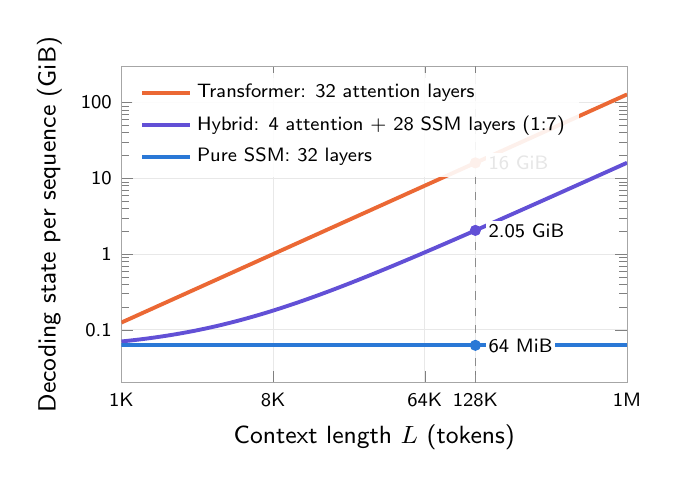
\begin{tikzpicture}
\begin{axis}[width=0.66\textwidth, height=5.6cm, xmode=log, ymode=log, log basis x=2,
  xmin=1024, xmax=1048576, ymin=0.02, ymax=300,
  xtick={1024,8192,65536,131072,1048576}, xticklabels={1K,8K,64K,128K,1M},
  ytick={0.1,1,10,100}, yticklabels={0.1,1,10,100},
  xlabel={Context length $L$ (tokens)}, ylabel={Decoding state per sequence (GiB)},
  grid=major, grid style={line width=0.3pt, draw=black!9}, axis line style={black!35},
  tick label style={font=\scriptsize\sffamily}, label style={font=\small\sffamily},
  legend style={font=\scriptsize\sffamily, draw=none, fill=white, fill opacity=0.9, text opacity=1, at={(0.02,0.98)}, anchor=north west, row sep=1pt},
  legend cell align=left]
\addplot[attn, line width=1.4pt, domain=1024:1048576, samples=2] {x*131072/1073741824};
\addlegendentry{Transformer: 32 attention layers}
\addplot[hyb, line width=1.4pt, domain=1024:1048576, samples=80] {x*16384/1073741824 + 28*2097152/1073741824};
\addlegendentry{Hybrid: 4 attention + 28 SSM layers (1:7)}
\addplot[ssm, line width=1.4pt, domain=1024:1048576, samples=2] {32*2097152/1073741824};
\addlegendentry{Pure SSM: 32 layers}
\draw[black!45, dashed, line width=0.5pt] (axis cs:131072,0.02) -- (axis cs:131072,300);
\node[font=\scriptsize\sffamily, fill=white, inner sep=1pt, anchor=west] at (axis cs:150000,16) {16 GiB};
\node[font=\scriptsize\sffamily, fill=white, inner sep=1pt, anchor=west] at (axis cs:150000,2.05) {2.05 GiB};
\node[font=\scriptsize\sffamily, fill=white, inner sep=1pt, anchor=west] at (axis cs:150000,0.0625) {64 MiB};
\addplot[only marks, mark=*, mark size=1.8pt, attn] coordinates {(131072,16)};
\addplot[only marks, mark=*, mark size=1.8pt, hyb] coordinates {(131072,2.0547)};
\addplot[only marks, mark=*, mark size=1.8pt, ssm] coordinates {(131072,0.0625)};
\end{axis}
\end{tikzpicture}
\caption{\label{fig:memory}Per-sequence decoding memory for an illustrative 8B-scale configuration (our calculation, not a measurement): 32 layers; attention with grouped-query KV of 8 heads $\times$ 128 dimensions; SSM layers with inner width 8192 and state size $N{=}128$; 16-bit storage. The KV cache grows linearly (128 KiB per token), the SSM state is constant, and the hybrid is dominated by its few attention layers beyond $\sim$4K tokens. Log--log axes; values at 128K tokens are annotated.}
\end{figure}

\subsection{The recall--memory trade-off}
\label{sec:recall}
The most consequential limitation of fixed-state models is information-theoretic rather than architectural. The following elementary counting argument, in the spirit of \citet{jelassi2024repeat}, makes this precise.

\begin{proposition}[Copying requires memory linear in length]
\label{prop:copy}
Let a causal model read a string $w\in\Sigma^n$ followed by a delimiter, and suppose everything it carries forward is a state of $b$ bits. If $n\log_2|\Sigma|>b$, then there exist two distinct strings that the model maps to the same state, and it fails to copy at least one of them.
\end{proposition}
\begin{proof}[Proof sketch]
There are $|\Sigma|^n=2^{n\log_2|\Sigma|}>2^b$ input strings but at most $2^b$ distinct states. By the pigeonhole principle, two strings $w\neq w'$ reach the same state. All subsequent outputs are a function of that state (and of the model's own outputs), so the continuations for $w$ and $w'$ are identical, and at least one is wrong.
\end{proof}

\noindent \citet{jelassi2024repeat} prove the complementary positive result (a two-layer Transformer can copy strings of exponential length) and observe that Transformers also \emph{learn} to copy far more sample-efficiently. \citet{arora2024based} trace a smooth Pareto frontier between recurrent state size and recall accuracy and show that simple linear attention combined with sliding windows (\textquotedblleft Based\textquotedblright) can move along it. Together with Eq.~\eqref{eq:crosstalk}, these results suggest a sharp interpretation of Generation~III. Better update rules (delta, gating, test-time optimizers) use a fixed budget of $d_kd_v$ numbers \emph{more efficiently}, by reducing interference and evicting stale associations. They cannot raise the budget. This is why we argue that the residual gap is a \emph{capacity} gap, not an optimization gap, and why hybrids---which restore a growing memory in a few layers---are the pragmatic answer rather than a temporary compromise.

\subsection{Expressivity and state tracking}
\label{sec:expressivity}
A second, independent axis concerns \emph{what can be computed} rather than \emph{what can be remembered}. \citet{merrill2024illusion} show that log-precision S4 and S6 (Mamba) layers, like Transformers, lie in the circuit class $\mathsf{TC}^0$. Unless $\mathsf{TC}^0=\mathsf{NC}^1$, they therefore cannot solve $\mathsf{NC}^1$-hard state-tracking problems such as composing permutations (the $S_5$ word problem), which underlie tracking chess moves, code execution or entity states. The recurrent form is no guarantee of recurrent power: a diagonal, non-negative transition can only rescale each coordinate monotonically. A one-dimensional example shows what negative eigenvalues buy. With $h_0=1$ and $h_t=a(x_t)h_{t-1}$, where $a(0)=1$ and $a(1)=-1$, we get $h_L=(-1)^{\sum_tx_t}$, which is exactly the parity of the input; with $a(\cdot)\in[0,1]$ no such sign flip exists. This is the intuition behind \citet{grazzi2025negative}. We can now order transitions into a hierarchy---scalar (Mamba-2, mLSTM) $\subset$ diagonal (Mamba, GLA) $\subset$ identity-plus-low-rank (DeltaNet, DeltaProduct) $\subset$ dense (nonlinear RNNs)---along which expressivity increases while parallel efficiency decreases. In our reading, the most productive recent work searches for the richest transition that remains chunk-parallelizable on tensor cores.

\subsection{Beyond language}
\label{sec:beyond}
SSMs predate their use in language: Generation~I was strongest on continuous signals. In genomics, HyenaDNA \citep{nguyen2023hyenadna} models up to one million nucleotides at single-nucleotide resolution. Vision is more nuanced. Vision Mamba \citep{zhu2024vim} and VMamba \citep{liu2024vmamba} must impose a 1-D causal scan order on 2-D data and compensate with bidirectional or multi-directional scans. Their efficiency advantage over attention appears mainly at high resolution, where token counts are large. We view this as evidence that the inductive bias of a causal scan is natural for genuinely sequential data and is a workaround elsewhere.

\begin{table}[t]
\centering
\caption{Strengths, limitations and the work that addressed them. The right-most column shows the bottleneck-to-fix chain underlying Fig.~\ref{fig:taxonomy}.}
\label{tab:critique}
\footnotesize
\renewcommand{\arraystretch}{1.2}
\begin{tabularx}{\textwidth}{@{}>{\raggedright\arraybackslash}p{2.35cm} >{\raggedright\arraybackslash}X >{\raggedright\arraybackslash}X >{\raggedright\arraybackslash}p{2.9cm}@{}}
\toprule
\textbf{Method} & \textbf{What it nails} & \textbf{Where it falls short} & \textbf{Addressed by} \\
\midrule
S4 \citep{gu2022s4} & Principled long memory; convolutional training; first to solve Path-X & Time-invariant (no content selection); complex NPLR machinery & S4D/DSS (simplicity); Mamba (selectivity) \\
S4D, DSS, LRU & Diagonal recurrences match S4 with far simpler code & Still time-invariant; weak on language & Mamba, GLA \\
H3, Hyena & Data-controlled gating brings SSMs/convolutions closer to attention on language & Recall gap (MQAR); long convolutions cost $\bigO(L\log L)$ and decode poorly & Based, Mamba \\
RWKV, RetNet & Parallel training with $\bigO(1)$ decoding, scaled to billions of parameters & Fixed decay cannot decide what to forget & GLA, Mamba \\
Mamba & Input-dependent selection; fast hardware-aware scan; strong small-scale LM & Scan not tensor-core friendly ($N{=}16$); recall and state-tracking limits & Mamba-2; DeltaNet; hybrids \\
Mamba-2, GLA & Matmul-friendly chunking; larger states; duality with attention & Decay erases all associations at once; no targeted overwrite & DeltaNet, Gated DeltaNet \\
DeltaNet & Error-correcting writes reduce interference; better recall & No fast global forgetting & Gated DeltaNet \\
Gated DeltaNet & Combines decay and delta; strong LM and retrieval; adopted in production hybrids & Fixed capacity (Prop.~\ref{prop:copy}); positive eigenvalues by default & Negative eigenvalues, DeltaProduct; hybrids \\
TTT, Titans & Expressive nonlinear memory learned at test time & Harder to parallelize; less mature large-scale evidence & Open \\
Hybrids & Best quality--efficiency trade-off observed in practice & Retain a quadratic, growing component; ratios found by trial and error & Open (Section~\ref{sec:future}) \\
\bottomrule
\end{tabularx}
\end{table}

\section{Open Problems and Future Directions}
\label{sec:future}
We close with the questions we consider most important, ordered roughly from those likely to yield to engineering to those that need new ideas.

\paragraph{1. Adaptive memory size.} Every model in Table~\ref{tab:unified} fixes the state size before seeing the data, whereas attention's memory grows with the context. Proposition~\ref{prop:copy} says that neither extreme is right for every task. A natural next step is memory whose size grows \emph{sublinearly}---for example logarithmically, through multi-resolution or hierarchical states that keep recent context finely and distant context coarsely---or whose size is allocated by the model itself according to the predicted recall demand. We expect such \textquotedblleft elastic\textquotedblright{} memories to blur the boundary between recurrent layers and hybrids.

\paragraph{2. A theory of hybridization.} Independent groups converged on remarkably similar ratios---1:7 in Jamba and MiniMax-01, about 8\% attention in Nemotron-H, 3:1 recurrent-to-attention in Qwen3-Next and Kimi Linear---but by search rather than by principle. The capacity view of Section~\ref{sec:recall} suggests a testable hypothesis: the attention fraction a model needs is governed by the \emph{recall demand of the data distribution} (how many distinct, exactly-needed facts per context), not by model size. Placement (early, middle or late layers), the type of attention (global or sliding-window) and the sharing of KV caches across layers are equally under-explored.

\paragraph{3. Richer transitions that remain parallel.} The hierarchy of Section~\ref{sec:expressivity} frames a concrete search problem: find transition families that are closed under multiplication (so chunks compose), admit compact representations (so chunks run on tensor cores), and contain negative or rotational eigenvalues (so states can be tracked). Products of Householder matrices are one answer. Block-diagonal, permutation-augmented or low-rank-plus-diagonal families are obvious candidates that, to our knowledge, have not been systematically compared at scale.

\paragraph{4. What should the memory optimize?} The test-time-regression view turns architecture design into the choice of an inner objective and optimizer. So far that choice has been hand-designed (squared loss, one step of SGD, sometimes momentum). Meta-learning the inner objective, using second-order or normalized inner optimizers, and drawing on continual-learning results on catastrophic interference are natural directions. One caveat: every added inner-loop sophistication must survive the parallelization constraint above.

\paragraph{5. Evaluation that measures the right thing.} Perplexity is a poor proxy here: Zoology showed that a small set of recall tokens dominates the perplexity gap, and LRA rewards inductive biases that matter little for language. We advocate reporting, alongside standard benchmarks, (i) synthetic recall (MQAR) at multiple state sizes, (ii) state-tracking suites (parity, permutation composition), (iii) long-context retrieval and aggregation such as RULER \citep{hsieh2024ruler}, and (iv) end-to-end serving metrics---throughput at fixed latency and batch size---instead of kernel-level speedups.

\paragraph{6. Systems for recurrent state.} A KV cache is an append-only log: it can be truncated, shared across requests with a common prefix, and rolled back after a rejected speculative draft. A recurrent state is a lossy summary that supports none of these for free. Prefix caching requires storing states at checkpoints, and speculative decoding requires state snapshots or recomputation \citep{wang2024mambainllama}. We expect serving-system support for state checkpointing and rollback to matter as much for adoption as any further architectural gain.

\paragraph{7. Interpretability and editing.} Under Eq.~\eqref{eq:unified}, the state is an explicit associative memory $\mS_t$ whose contents can, in principle, be probed with keys, edited with targeted delta updates, or transplanted between contexts. We consider this an under-appreciated opportunity: the same structure that limits capacity may make recurrent memories easier to inspect and control than KV caches.

\section{Conclusion}
\label{sec:conclusion}
Over five years, linear-time sequence modeling has evolved from structured time-invariant ODEs (Generation~I), through input-dependent selection and gating (Generation~II), to memories that perform explicit online regression at test time (Generation~III). A single recurrence, $\mS_t=\mathcal{T}_t(\mS_{t-1})+\beta_t\vv_t\vk_t\T$, organizes this progression, and structured state space duality shows that it sits on the same continuum as attention. Our analysis separates two limits that are often conflated: a \emph{capacity} limit, which no update rule can overcome with a fixed-size state, and an \emph{expressivity} limit, which richer transitions (negative eigenvalues, Householder products) can lift at some cost in parallelism. The industrial convergence on hybrids with roughly one attention layer per three to seven recurrent layers is, in this light, a principled division of labor rather than a stopgap: recurrent layers compress what can be compressed, and a few attention layers retain what must be recalled exactly. The open problems---adaptive memory, a theory of hybridization, expressive-yet-parallel transitions, better inner objectives, and honest evaluation---suggest that the most interesting work in this area is still ahead.

\clearpage
\bibliographystyle{apalike}
\bibliography{Paper_summaries}
\end{document}
